\BeginSection{Введение}
\begin{frame}[t]{Задача тематического моделирования}
\textbf{Дано:}
\begin{itemize}
    \item $D$ --- коллекция текстовых документов
    \item $W$ --- множество уникальных термов коллекции
    \item $n_{dw}$ --- число вхождений слова $w$ в <<мешок слов>> документа $d$
\end{itemize}

\medskip
\textbf{Найти:}
множество тем $T$ и два семейства распределений:
\smallskip
\begin{itemize}
    \item $p(w \cond t)$ --- распределения термов в темах (матрица $\Phi$)
    \item $p(t \cond d)$ --- распределения тем в документах (матрица $\Theta$)
\end{itemize}

\[
p(w \cond d) = \sum_{t \in T} p(w \cond t)p(t \cond d) = \sum_{t \in T} \phi_{wt}\theta_{td}
\]

\smallskip
\textbf{Критерий:} максимум правдоподобия либо максимум регуляризированного правдоподобия (правдоподобие складывается с некоторым числом взвешенных регуляризаторов $\sum \tau_i R_i$)

Получаем много гиперпараметров: список регуляризаторов, их коэффициенты, число тем $T$.
% \footnotetext{
% Воронцов К. В. Аддитивная регуляризация тематических моделей коллекций текстовых документов // Доклады РАН. 2014.}
\end{frame}


\begin{frame}[t]{Проблемы тематических моделей на практике}

С какими проблемами сталкиваются пользователи тематических моделей?
\begin{enumerate}
    \item{ Неустойчивость \begin{itemize}
        \item {Зависит от $T$ и других гиперпараметров}
    \end{itemize}}
    \item{ Мусорные темы \begin{itemize}
        \item {При помощи сглаживания/разреживания можно выделить мусор в специальные фоновые темы}
    \end{itemize}}
    \item{ Дублирующие темы \begin{itemize}
        \item {Регуляризатор декорреляции делает темы различными}
    \end{itemize}}
    \item{ Вводящие в заблуждение темы \begin{itemize}
        \item {Увы, регламент валидации не разработан}
    \end{itemize}}
    \item{ Неинтерпретируемые или плохо интерпретируемые темы \begin{itemize}
        \item {Увы, процедуры измерения интерпретируемости ненадёжны}
    \end{itemize}}
\end{enumerate}
В теории настройка гиперпараметров может устранить проблемы 3, 4, 5. Если существовали бы чёткие критерии для проблем 1 и 2,  то настройка гиперпараметров могла бы помочь и с ними.
\end{frame}
\note{
В теории именно настройка гиперпараметров отличает плохую модель от хорошей.

Что такое плохая тематическая модель?
Ну, я выделю ряд проблем важных на практике. Пойду снизу вверх.

Неустойчивость --- не позволяет говорить о какой-то определённой модели. Связана как минимум с числом тем. Разреживание позволяет уменьшить число валидных локальных максимумов.

Мусорные темы --- совсем избавиться от них нельзя, но в теории их можно изолировать.

Дублирующие темы --- плохо потому что не даёт исследователю информации. Стандартный регуляризатор декорреляции хорошо с этим справляется.

Вводящие в заблуждение темы --- нужны инструменты визуализации.

Неинтерпретируемые --- нужны критерии качества.
}

% Проблема: никто не умеет подбирать гиперпараметры. В статье\footnote{Chen T. H., Thomas S. W., Hassan A. E. A survey on the use of topic models when mining software repositories – 2016.} сделали обзор 167 статей: 45\% работ не указывает использованное значение $T$ вовсе, 33\% приводит его без разъяснений о том, как оно было выбрано, 9\% используют перебор различных значений.

\begin{frame}[t]{Задачи диссертационного исследования}
\small
\textbf{Задачи:}
\begin{enumerate}
    \item Реализация, эмпирическое исследование и улучшение автоматически вычисляемых критериев интерпретируемости тематических моделей, в том числе нового критерия внутритекстовой когерентности.
\end{enumerate}

\begin{figure}
    %\begin{tabular}{p{7.5cm}p{3.5cm}}
        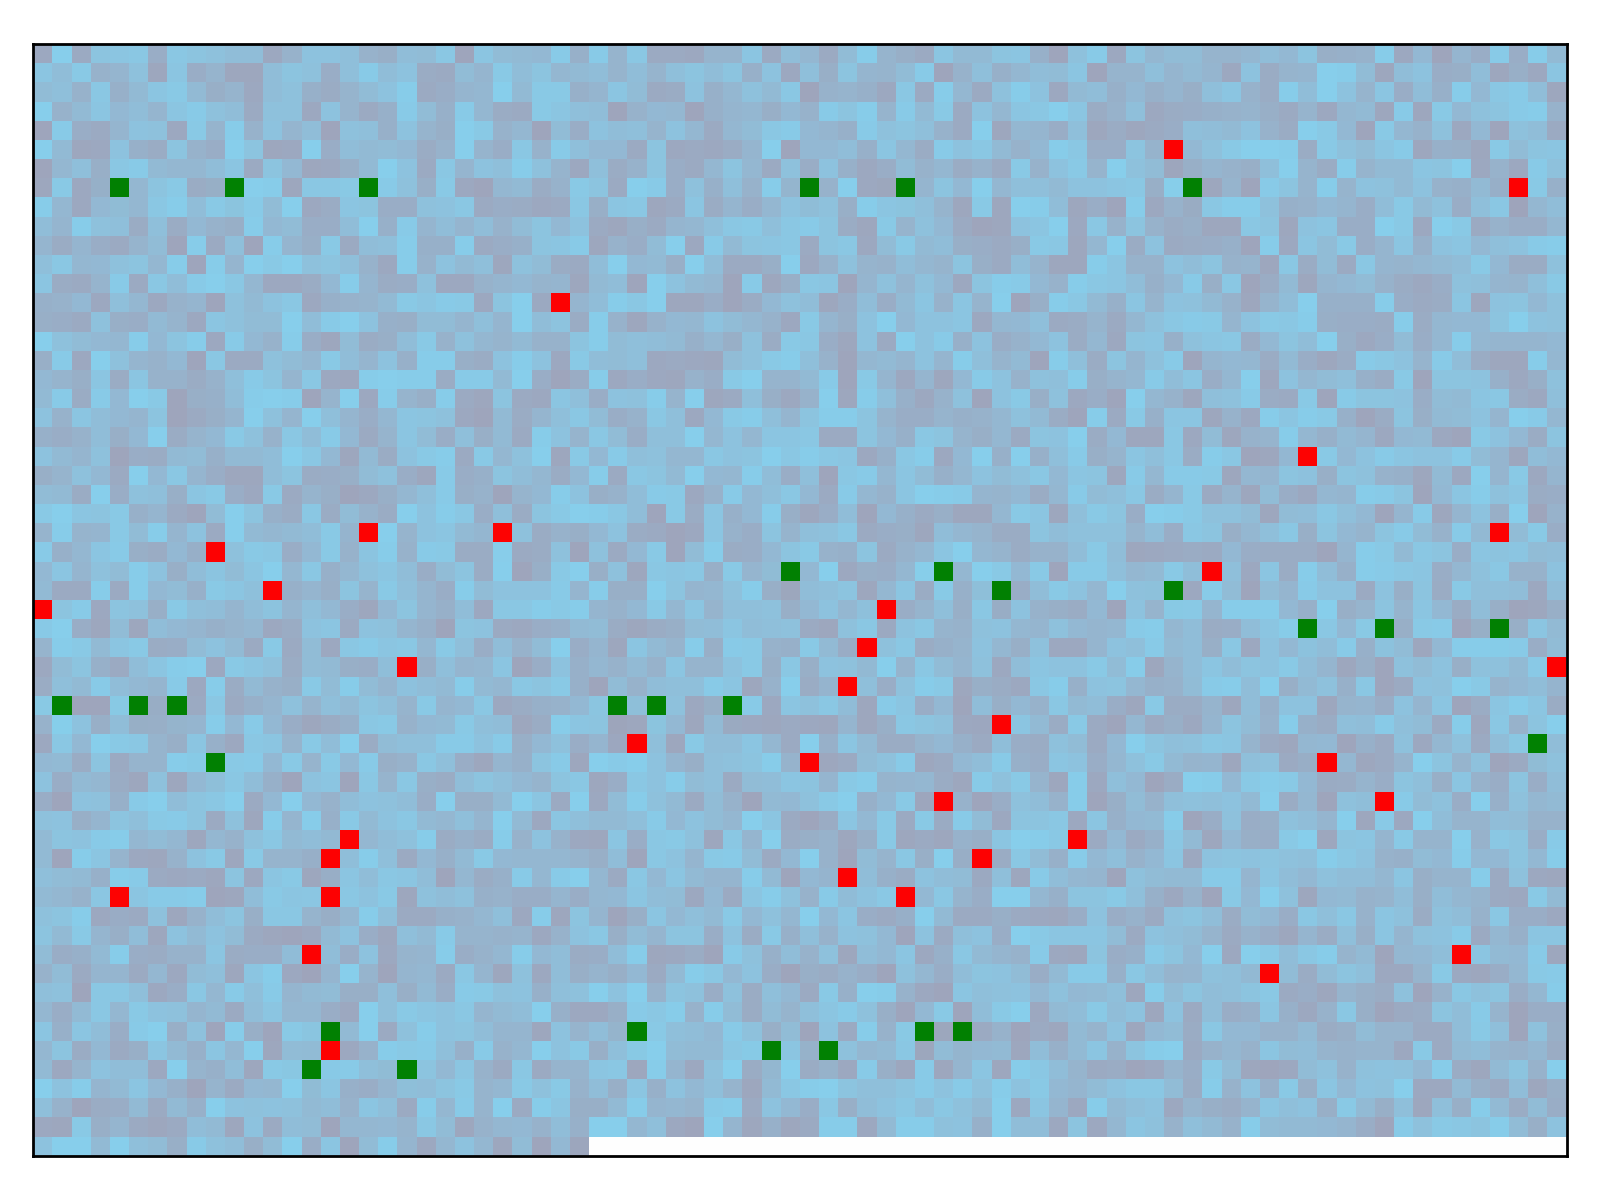
\includegraphics[width=0.5\textwidth]{doc11358_topic0.png} %&
        % 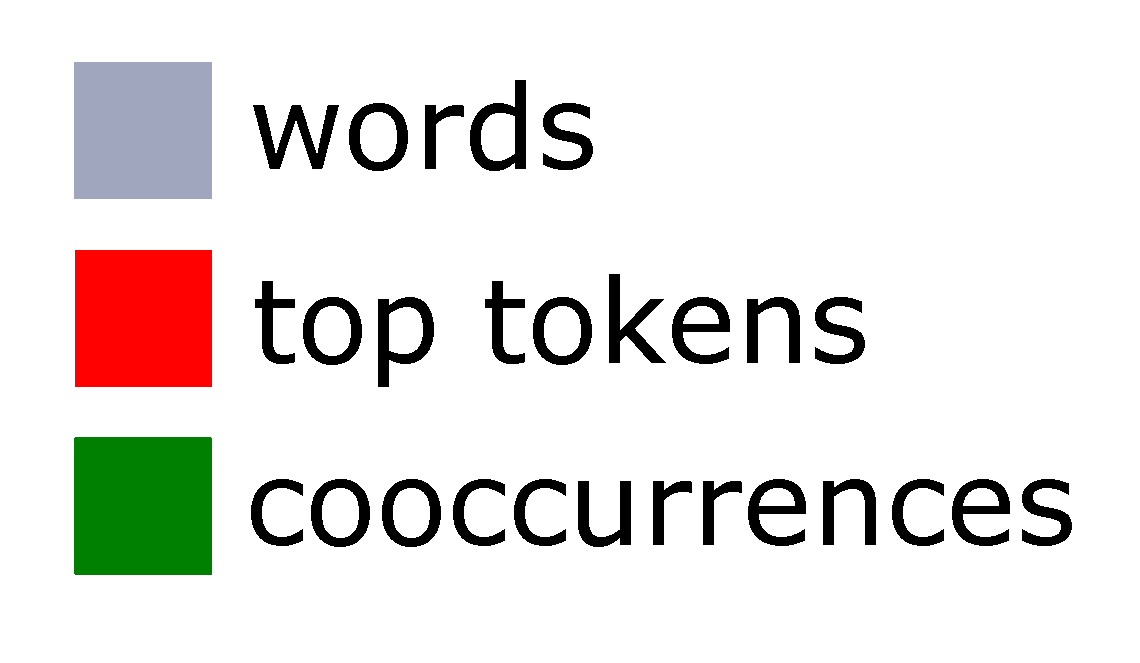
\includegraphics[width=0.25\textwidth]{legend.eps} \\
    %\end{tabular}
\end{figure}
\vspace{-7pt}
Словопозиции обозначены серо-синим цветом, словопозиции верхних слов показаны красным цветом, зелёным цветом показаны словопозиции, имеющие ненулевой вклад в расчёт когерентности (т.е. попадающие в скользящее окно вместе с другим верхним словом).
\normalsize

\end{frame}
\begin{frame}[t]{Задачи диссертационного исследования}
% \begin{frame}{Внутритекстовая когерентность}
\begin{figure}
   \centering
    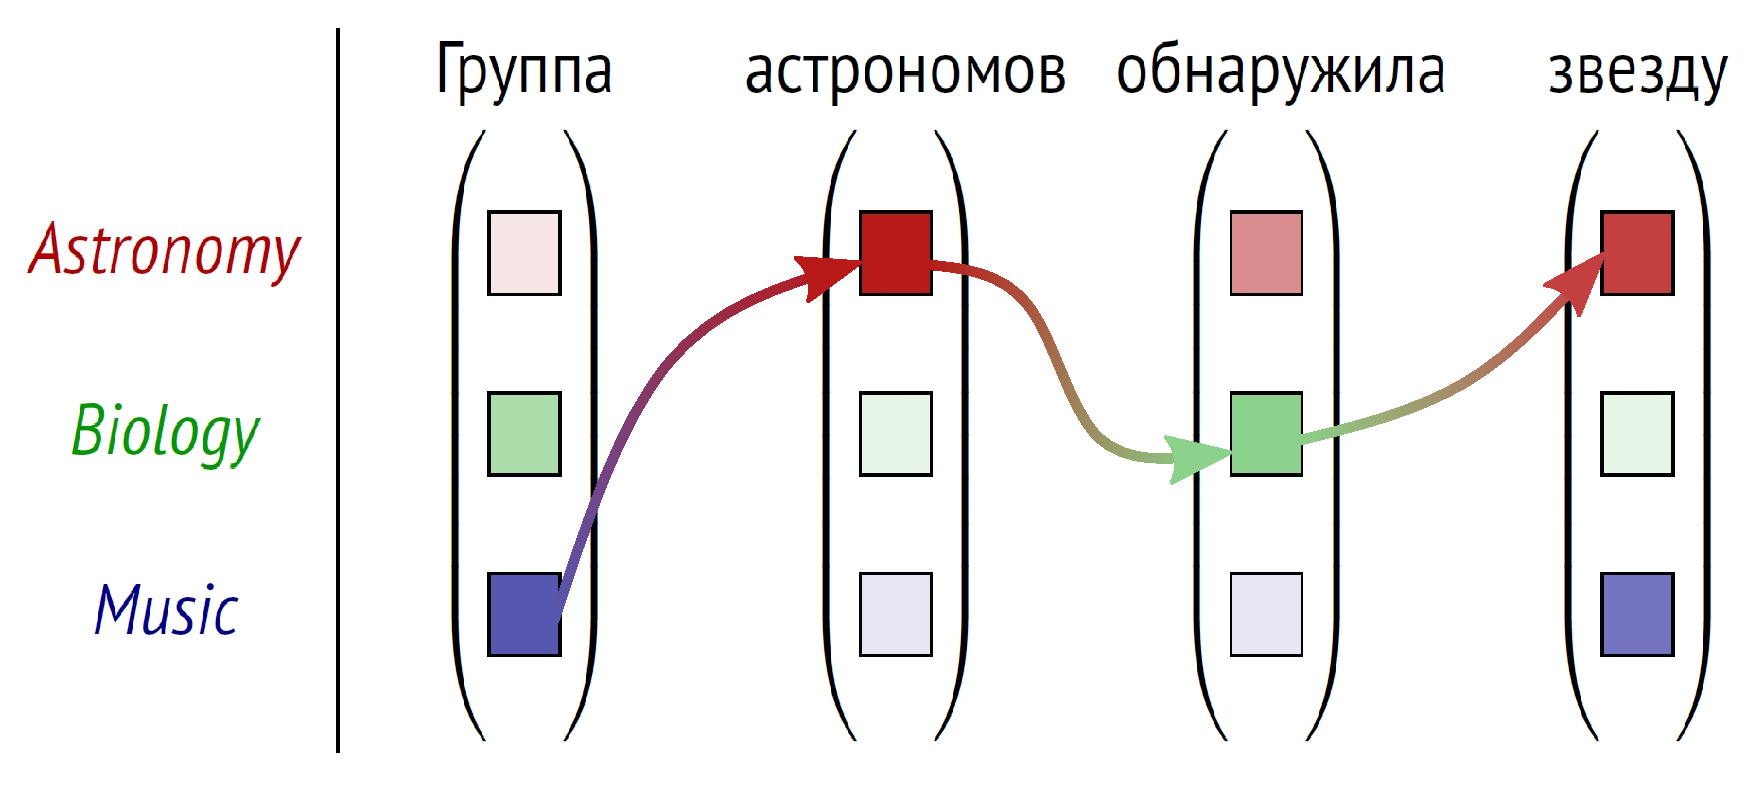
\includegraphics[width=0.8\textwidth, height=0.3\textheight]{astronomers_focon.eps} % .eps image is wrong scaled
\end{figure}

Идея: выделить все соседние слова текста и анализировать их распределение $\phi_{wt}$.\\
\medskip
(вместо того, чтобы выделять небольшое множество слов при помощи $\phi_{wt}$ и затем анализировать, как эти слова встречаются в тексте)
\bigskip
\small{(таким образом, измерение интерпретируемости остаётся открытой проблемой)}
\end{frame}


\begin{frame}[t]{Задачи диссертационного исследования}
% \begin{frame}[t]{Основная идея диссертационной работы}

\begin{figure}[ht]
    \centering
    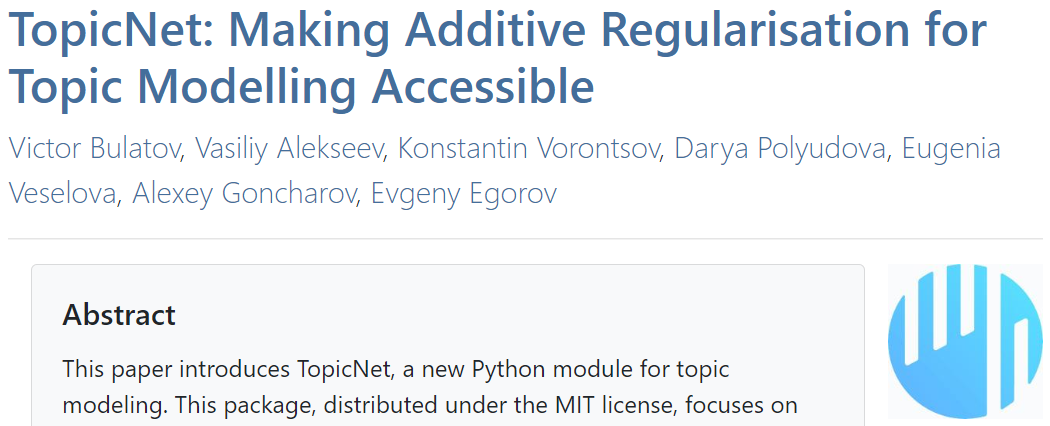
\includegraphics[width=0.99\textwidth]{Presentation/images/topicnet_paper.png}
\end{figure} 

\bigskip

\textbf{Цель:} разработка технологии построения интерпретируемых  тематических моделей, применимых для решения широкого класса задач тематического моделирования.

\bigskip
\small{(Это задачи 2-5 диссертационного исследования)}

\end{frame}




% \begin{frame}[t]{Доступность тематических моделей}

% Таким образом, принятые методологии перекладывают ответственность за подбор гиперпараметров на исследователя; при этом процедура подбора остаётся нерегламентированной, что создаёт высокий барьер входа для неспециалистов. 

% В~обзорной монографии \cite{fntir2017applications} подчёркивается важность снижения порога входа и более жёсткой регламентации процесса моделирования: <<первоочередная исследовательская задача в тематическом моделировании... сделать его более доступным>>.

% \end{frame}

\BeginSection{Методология построения ТМ в библиотеке TopicNet}

\begin{frame}{Дерево эксперимента в библиотеке TopicNet}

\begin{figure}[ht]
\small
Каждое ребро --- некое преобразование: модель-предок $\rightarrow$ модель-потомок. Все рёбра одного
уровня описывают преобразования из одного и того же семейства,
различающиеся лишь набором параметров.\\
    \centering
    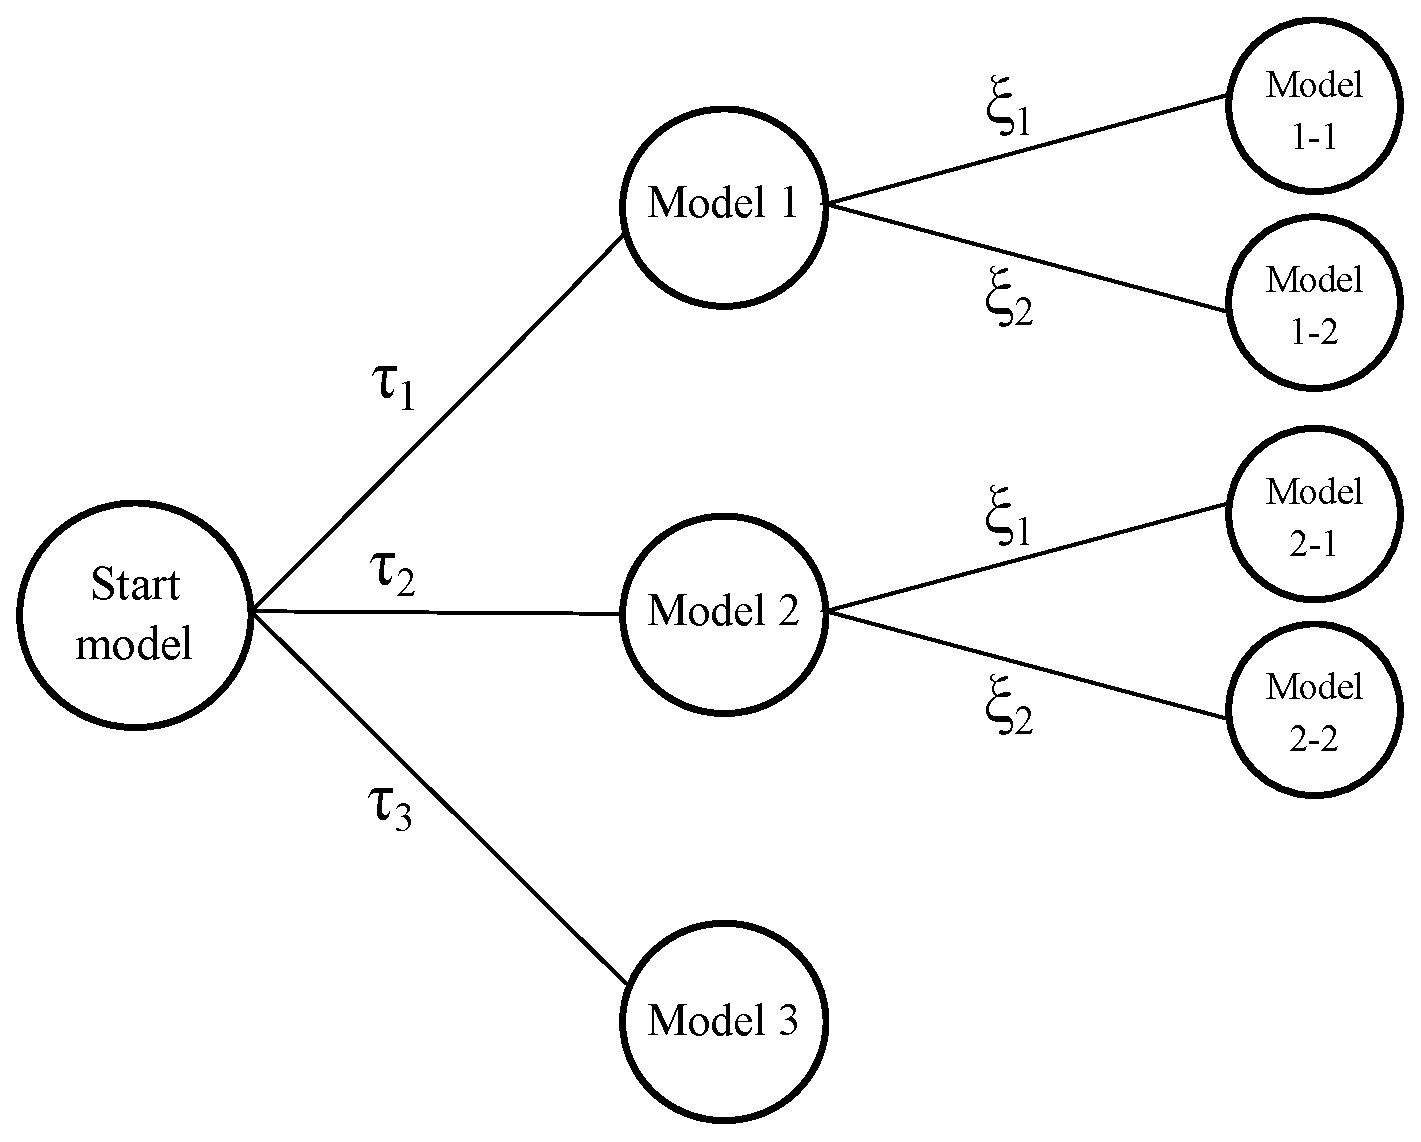
\includegraphics[width=0.6\textwidth]{training_scheme_example.eps}
\end{figure} 
        Первый этап: регуляризатор с $\tau \in \{\tau_1, \tau_2, \tau_3\}$.\\
        Лучшими оказываются \emph{Model 1} и \emph{Model 2}, они проходят на второй этап. К ним применяется другой регуляризатор с $\xi \in \{\xi_1, \xi_2\}$.
\normalsize
\end{frame}

\begin{frame}[t]{Cube: чертёж и инкубатор}

Класс \texttt{Cube}~--- базовый класс, его наследники должны реализовать две важные функции.

\textit{Спецификация}: пользователь задаёт параметры, нужно построить многомерное пространство поиска.

\begin{minipage}{0.39\textwidth}
{\small \texttt{\textcolor{blue}{\_\_init\_\_}(\\
\hphantom{\ \ \ \ }tau\_min,\ tau\_max,\\ 
\hphantom{\ \ \ \ }xi\_combination\_mode,\\
\hphantom{\ \ \ \ }eta\_array\\
)}}
\end{minipage}
\begin{minipage}{0.05\textwidth}
\scalebox{2}{$\rightarrow$}
\end{minipage}
\begin{minipage}{0.45\textwidth}
\begin{tikzpicture}
   \pic [text=blue!75!cyan] at (0,1) {annotated cuboid={
   width=300, height=200, depth=200, scale=.007, 
   xstring={$\{\tau_1,\tau_2,\tau_3\}$}, 
   ystring={$\{\xi_1,\xi_2\}$}, 
   zstring={$\{\eta_1,\eta_2\}$},, 
   }};
\end{tikzpicture}
\end{minipage}
  
% Эксперимент --- цепочка кубов.

\textit{Применение}: есть модель и точка в пространстве поиска, нужно построить модель-потомка.

\begin{minipage}{0.1\textwidth}
    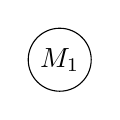
\begin{tikzpicture}
        \draw (0,0) circle [radius=0.4] node {$M_1$};
    \end{tikzpicture}
\end{minipage}
\begin{minipage}{0.4\textwidth}
    \begin{tikzpicture}
       \pic [text=blue!75!cyan] at (0,1) {annotated cuboid={
       width=300, height=200, depth=200, scale=.007,
          xstring=, ystring=, zstring=, 
       }};
       \draw[fill,blue] (-1,0)--(1.5,1) node[above]{$(\tau_1,\,\xi_2,\,\eta_1)$};
       \draw (-1,0) circle[radius=2pt];
    \end{tikzpicture}
\end{minipage}
\begin{minipage}{0.05\textwidth}
    \scalebox{2}{$\rightarrow$}
\end{minipage}
\begin{minipage}{0.2\textwidth}
    
\includegraphics[width=\textwidth]{Presentation/images/incuber.png}
\end{minipage}
\begin{minipage}{0.1\textwidth}
    \scalebox{2}{$\rightarrow$}
\end{minipage}
\begin{minipage}{0.1\textwidth}
    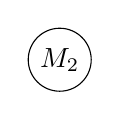
\begin{tikzpicture}
        \draw (0,0) circle [radius=0.4] node {$M_2$};
    \end{tikzpicture}
\end{minipage}


% Regularizer Modifier Cube: <<применить к модели регуляризатор с произвольными параметрами и запустить процесс обучения модели на какое-то количество итераций>>.

% Creator Cube: <<инициализировать модель произвольными параметрами>>.

\end{frame}

\begin{frame}{Отбор моделей в библиотеке TopicNet}

Отбор моделей должен быть многокритериальным. Для удобства в TopicNet введён специальный язык отбора моделей:

\begin{figure}[ht]
% \footnotesize
\raggedright
\texttt{TopicKernel@word.average\_contrast > 0.95 * MAXIMUM( \\
\hphantom{\ \ \ \ \ \ \ \ }TopicKernel@word.average\_contrast) \\
\hphantom{\ \ } and PerplexityScore@all < 1.1 * MINIMUM( \\
\hphantom{\ \ \ \ \ \ \ \ }PerplexityScore@all) \\
\hphantom{\ \ } and SparsityPhiScore@word -> max\\
\hphantom{\ \ } COLLECT 3} \\
\label{DSL-example}
\end{figure} 
	
%\begin{lstlisting}
%S -> <Expr> | <Expr> <Clct>
%<Clct> -> COLLECT <Int>
%<Expr> -> <Expr> AND <Expr>
%<Optr> -> less | eq | great
%<Expr> -> <Literal> <Optr> <Number>
%<Expr> -> <Literal> to MIN | <Literal> to MAX
%<Literal> -> <ScoreName> | model<ParameterName>
%\end{lstlisting} 

\bigskip
Поддержка пользовательским критериев качества:\\
\medskip
\texttt{model.num\_topics == 10 and SparsityPhiScore\@word > MEDIAN(SparsityPhiScore\@word) and MyCustomScore -> max}\\
\medskip
Так реализованы \texttt{BleiLaffertyScore}, \texttt{LogLift}, попарные расстояния между темами.
\end{frame}

\begin{frame}{Другие возможности TopicNet}
\begin{itemize}
    \item{Рецепты моделирования: задание эксперимента при помощи текста}
    \begin{itemize}
        \item (есть Baseline Recipe, основанный на стратегии Мурата Апишева) 
    \end{itemize}
    \item{стратегии обхода пространства поиска (гиперкуба параметров)}
    \begin{itemize}
        \item (например: начинаем с $\tau=0$, увеличиваем коэффициент линейно на 0.01 до тех пор, пока перплексия новой модели не будет слишком большой.) 
    \end{itemize}
    \item{Сохранение дерева эксперимента на диск}
    \item{Поддержка пользовательских регуляризаторов}
    \item{Средства визуализации}
\end{itemize}

\end{frame}

\BeginSection{Таксономия обращений и относительные коэффициенты}


\begin{frame}{Таксономия обращений}
	Дано: большая коллекция диалогов между клиентом и оператором.\\
	
	Найти: иерархию интентов, входящих в коллекцию. \\
	
	Критерии: \begin{itemize}
	    \item Интерпретируемая тематическая модель
	    \item Иерархическая модель, два уровня.
	    \item  Темы первого уровня описывают субъект диалога
	    \item  Темы второго уровня должны описывать действие, в котором заинтересован пользователь.
	    \item  \emph{Стратегия построения модели должна переноситься на похожие коллекции}
	\end{itemize}

\end{frame}

\begin{frame}{Дополнительные модальности}


Используется пять модальностей:
\begin{itemize}
    \item \texttt{@lemmatized} (просто слова)
    \item \texttt{@verb\_lemmatized} (слова-глаголы)
    \item \texttt{@noun\_lemmatized} (слова-существительные и слова-прилагательные)
    \item \texttt{@theme\_ngramms} ($n$-грамы с существительными и без глаголов)
    \item \texttt{@verb\_ngramms} ($n$-грамы с глаголами)
\end{itemize}

%{\footnotesize
%(информативные $n$-грамы выделены с помощью модифицированного алгоритма TopMine)}

\bigskip
Формула общего правдоподобия для мультимодального случая:

\[
L(\Phi^m, \Theta) = \sum_m \tau_m \sum_{d\in D} \sum_{w \in W^m} n_{dw} \ln p(w \cond d) \rightarrow \max, 
\]

где коэффициенты $\tau_m$ показывают \textit{вес} модальности $m$. 

% Проинтерпретируем это выражение как введение $M-1$ дополнительного регуляризатора $\Theta$ с коэффициентами $\tau_m$. Тогда $\sum_{d\in D} r_{id}$ тоже выражается через константы, известные ещё на этапе построения коллекции:

%\[
%\tau_m = \lambda_m \frac{n}{\sum_d n_d^{(m)}} \iff
%\lambda_m = \tau_m \frac{\sum_d n_d^{(m)}}{n}
%\]

\end{frame}


\begin{frame}[t]{Относительные коэффициенты регуляризации}

Регуляризованное правдоподобие:
\[
    \sum_{d \in D} \sum_{w \in d} n_{dw} \mathrm{ln} \sum_{t \in T} \phi_{wt} \theta_{td} + \sum_{i} \tau_i R_i(\Phi, \Theta)
    \rightarrow \underset{\Phi, \Theta}{\mathrm{max}}
\]
Общие формулы M-шага:
\[
\theta_{td} = \norm_{t \in T} \Bigg(
    n_{td} + \sum_{i=1}^k \tau_i \theta_{td} \frac{\partial R_i}{\partial \theta_{td}}
\Bigg), \quad \phi_{wt} = \norm_{w \in W}\Bigg(
    n_{wt} + \sum_{i=1}^k \lambda_i 
    \phi_{wt} \frac{\partial R_i}{\partial \phi_{wt}}
\Bigg)
\]

\small
Идея: просуммировать каждое слагаемое по всем документам (для $\Theta$) или темам (для $\Phi$); отнормировать слагаемые на эту сумму. Тогда вместо $\tau_i$ будет  $\lambda_i$ - относительный коэффициент регуляризации, показывающий, \emph{во сколько раз} соответствующий регуляризатор влияет на оценку матриц больше, чем коллекция.

Случай $\phi_{wt}$ реализован в BigARTM, случай $\theta_{td}$~--- нет (поскольку $r_{id}$ недоступен при параллельной реализации).

\footnotetext{
Воронцов К. В. Аддитивная регуляризация тематических моделей коллекций текстовых документов // Доклады РАН. 2014.}

\end{frame}

\begin{frame}{Сглаживание, разреживание и веса модальностей}
Для некоторых важных случаев формула существенно упрощается!

\begin{table}[]
\begin{tabular}{l|c|c|}
         & \multicolumn{2}{c}{Управляющий параметр}                                                                                                      \\ \hline
         & $\tau$                                          & $\lambda$                                                                                   \\ \hline 
         &    &          \\[-5pt]
$\Phi$   & $\phi_{wt} = \norm_{w \in W}\Bigg(n_{wt} + \tau\Bigg)$    & $\phi_{wt} = \norm_{w \in W}\Bigg(n_{wt} + \lambda {\color{red}\frac{n}{|W||T|}}\Bigg)$    \\[15pt] \hline
         &    &          \\[-5pt]
$\Theta$ & $\theta_{td} = \norm_{t \in T} \Bigg(n_{td} + \tau\Bigg)$ & $\theta_{td} = \norm_{t \in T} \Bigg(n_{td} + \lambda {\color{red}\frac{n}{|D| |T|}}\Bigg)$ \\[15pt]  \hline
         &    &          \\[-5pt]
$\tau_m$ & $\theta_{td} = \norm_{t \in T} \Bigg(n_{td} + \tau n_{td}^{(m)}\Bigg)$ & $\theta_{td} = \norm_{t \in T} \Bigg(n_{td} + \lambda  {
    \color{red}\frac{n}{\sum_d n_d^{(m)}}
    } n_{td}^{(m)}\Bigg)$ \\[15pt]  \hline
\end{tabular}
\end{table}
Вывод: в этих случаях абсолютные коэффициенты и относительные эквивалентны. В частности, можно вычислить абсолютный коэффициент сглаживания $\Theta$, эквивалентный заданному относительному.
\end{frame}


\begin{frame}[t]{Решение. Полученные темы для двух коллекций}
% Веса модальностей \emph{относительные} и разные на двух уровнях. \\[-15pt]
%\\[-15pt]
\begin{table}[!t]
\begin{tabular}{|l|l|l|}\hline
                & Вес на первом уровне & Вес на втором уровне \\ \hline
\texttt{@lemmatized}     & 0.5                  & 0.5                  \\ \hline
 \texttt{@theme\_ngramms}   & 0.5                  & 0.5                  \\ 
\texttt{@noun\_lemmatized} & \textbf{0.5}                  & \textbf{0.1}                 \\ \hline
\texttt{@verb\_ngramms}    & \textbf{0.1}                  & \textbf{1}                    \\ 
\texttt{@verb\_lemmatized} & \textbf{0.1}                  & \textbf{1}                    \\ \hline
\end{tabular}
\end{table}

\footnotesize
\begin{table}[!h]
\begin{tabularx}{\textwidth}{|X|X|}
  \hline
  \textbf{Тарифный план} & \textbf{Запись на приём к врачу} \\
  \hline
  \textsl{Как \textbf{сменить} тарифный план?} &   \textsl{Как \textbf{записать} на приём ребёнка?}\\
  \textsl{Когда \textbf{произошло изменение} тарифного плана?} &   \textsl{Почему я \textbf{не могу записаться} на приём?}\\
  \textsl{Как часто можно \textbf{менять тарифный план}?} &  \textsl{\textbf{Не могу найти} в списке поликлинику №X?} \\
  \textsl{Когда \textbf{вступят в силу изменения} тарифного плана?} &    \textsl{Почему в списке \textbf{отсутствует специалист} X?} \\
  \textsl{Почему у меня \textbf{не получается изменить} тарифный план?} & \textsl{Как \textbf{отменить запись}?}\\
  \hline
\end{tabularx}
\caption{Различные подтемы темы верхнего уровня}
\label{topic_subtopic}
\end{table}
\normalsize

\end{frame}


\BeginSection{Качество тематических моделей с параметрами <<по умолчанию>>}


\begin{frame}{Конкуренты и <<параметры по умолчанию>>}

\begin{table}[h]
\begin{tabular}{|l|l|l|}
\hline
           & \multicolumn{1}{c|}{\begin{tabular}[c]{@{}c@{}}Jaccard measure\\ of topic dissimilarity\end{tabular}} & \multicolumn{1}{c|}{\begin{tabular}[c]{@{}c@{}}Average topic\\ coherence\end{tabular}} \\ \hline
TopicNet   & \textbf{0.00169}                                                                                               & -2.551                                                                                 \\ \hline
Gensim LDA & 0.01374                                                                                               & -2.747                                                                                 \\ \hline
STTM DMM   & 0.37541                                                                                               & -2.726                                                                                 \\ \hline
STTM PTM   & 0.02485                                                                                               & \textbf{-2.510}                                                                                 \\ \hline
STTM WNTM  & 0.01997                                                                                               & -3.572                                                                                 \\ \hline 
\end{tabular}
\caption{Сравнение качества различных моделей, построенных при помощи различных программных средств}
\end{table} 



\end{frame}


\begin{frame}{Функциональная зависимость $\Theta = f(\Phi)$}

Матрица $\Theta$ является менее важной, чем $\Phi$. На практике она часто не хранится в явном виде, а восстанавливается <<на лету>>.

\begin{itemize}
\item Оценка интерпретируемости: обычно используется только матрица $\Phi$.

\item Динамическое расширение коллекции документов: сильно увеличивается $|D|$, $|W|$ растёт медленнее.

\item Пакетный EM-алгоритм: разные документы обрабатываются разными потоками. Используется $\theta_d$, а не матрица $\Theta$ целиком.
\end{itemize}

\bigskip
По этим соображениям естественно рассмотреть зависимость $\Theta = f(\Phi)$, где $f$ --- одна итерация M-шага, восстанавливающая $\Theta$ с фиксированной $\Phi$.

\end{frame}

\begin{frame}[t]{$\Theta$ может скомпенсировать <<плохую>> $\Phi$}

Коллекция из 3 документов: 
\begin{figure}[t]
\begin{minipage}[t]{0.4\textwidth}
	\medskip
\begin{itemize}
    \item \texttt{herbs and spices}
    \item \texttt{spices and medicine}
    \item \texttt{herbs and medicine}
\end{itemize}
	\end{minipage}
	% $\qquad\quad$
	\begin{minipage}[t]{0.4\textwidth}
\begin{center}
\begin{tabular}{l|llll}
$n_{dw}$   & and & herbs & spices & medicine \\ \hline
doc1       & 1   & 1     & 1      & 0        \\
doc2       & 1   & 0     & 1      & 1        \\
doc3       & 1   & 1     & 0      & 1      
\end{tabular}
\end{center}

\end{minipage}
\end{figure}

Существуют решения с зашумлённой $\Phi$ (например, <<and>> во всех темах), недостатки которой  <<спрятаны>>  при помощи нулей в $\Theta$:
\small
\begin{minipage}[t]{0.4\textwidth}
\[
\Phi =
\begin{pmatrix}
0.044 & 0.488 & 0.488 & 0.281 \\
0.956 & 0     & 0     & 0     \\
0     & 0     & 0.512 & 0.279 \\
0     & 0.512 & 0     & 0.44  \\
\end{pmatrix},
\]
	\end{minipage}
	$\qquad\quad$
	\begin{minipage}[t]{0.4\textwidth}
\[
\Theta =
\begin{pmatrix}
0.349 & 0     & 0.348 \\
0     & 0.008 & 0.652 \\
0.651 & 0.244 & 0     \\
0     & 0.748 & 0     \\
\end{pmatrix}.
\]
\end{minipage}
\bigskip
\[
\Phi \cdot \Theta \approx \frac{1}{3} n_{dw}
\]
\normalsize
\end{frame}

\begin{frame}[t]{EM-алгоритм при $\Theta=f(\Phi)$ [Ирхин, 2020]}
При наличии зависимости $\Theta = f(\Phi)$ получается другая оптимизационная задача:

\begin{equation} \label{eq:tEM}
L(\Phi, f(\Phi) ) + R(\Phi, f(\Phi) ) \to \max_{\Phi},
\end{equation}
\small
\begin{Theorem}
    Пусть функция $R(\Phi,\Theta)$ непрерывно дифференцируема, а $\Theta$ находится в функциональной зависимости от $\Phi$ согласно формуле    $\theta_{td}(\Phi)
    = \norm_{t\in T} \biggl( \sum_{w\in W} n_{dw} p_{tdw} \biggr)$.
    Тогда точка $\Phi$ локального максимума 
    удовлетворяет системе уравнений со вспомогательными переменными $h_w,\ \theta_{td},\ p_{tdw},\ c_{td},\ \gamma_{dw}$:
\[
    \phi_{wt} = \norm_{w\in W}
        \Biggl(\,
        \sum_{d\in D} n_{dw} p_{tdw} 
        + \sum_{d\in D} n_{dw} n_d^{-1} \phi_{wt}h_w (c_{td}-h_w\gamma_{dw}) 
        + 
            \phi_{wt} \frac{\partial{R}}{\partial{\phi_{wt}}}
        \Biggr)
\]
\end{Theorem}
\normalsize
\end{frame}

\begin{frame}[t]{Псевдорегуляризатор быстрой векторизации}
\begin{minipage}[t]{0.99\textwidth}

\begin{align*}
    \phi_{wt} = \norm_{w\in W}
        \Biggl(\,&
        \sum_{d\in D} n_{dw} p_{tdw} \\
        + &\underbrace{\sum_{d\in D} n_{dw} n_d^{-1} \phi_{wt}h_w (c_{td}-h_w\gamma_{dw})}_{
            \let\scriptstyle\textstyle
            \substack{\textup{очень похоже на регуляризатор}}
        } \\ 
        + &\underbrace{
            \phi_{wt} \frac{\partial{R}}{\partial{\phi_{wt}}}
          }_{
          \let\scriptstyle\textstyle
            \substack{\textup{регуляризатор}}
        }
        \Biggr)
\end{align*}
\end{minipage}

Вывод: обучение можно <<сэмулировать>> внутри BigARTM, введя фиктивный псевдорегуляризатор и положив \texttt{num\_document\_passes~=~1}.

\end{frame}


\begin{frame}{Влияние на тематическую модель}

\begin{figure}
\setlength\tabcolsep{0pt} % default value: 6pt
\begin{tabular}{cc}
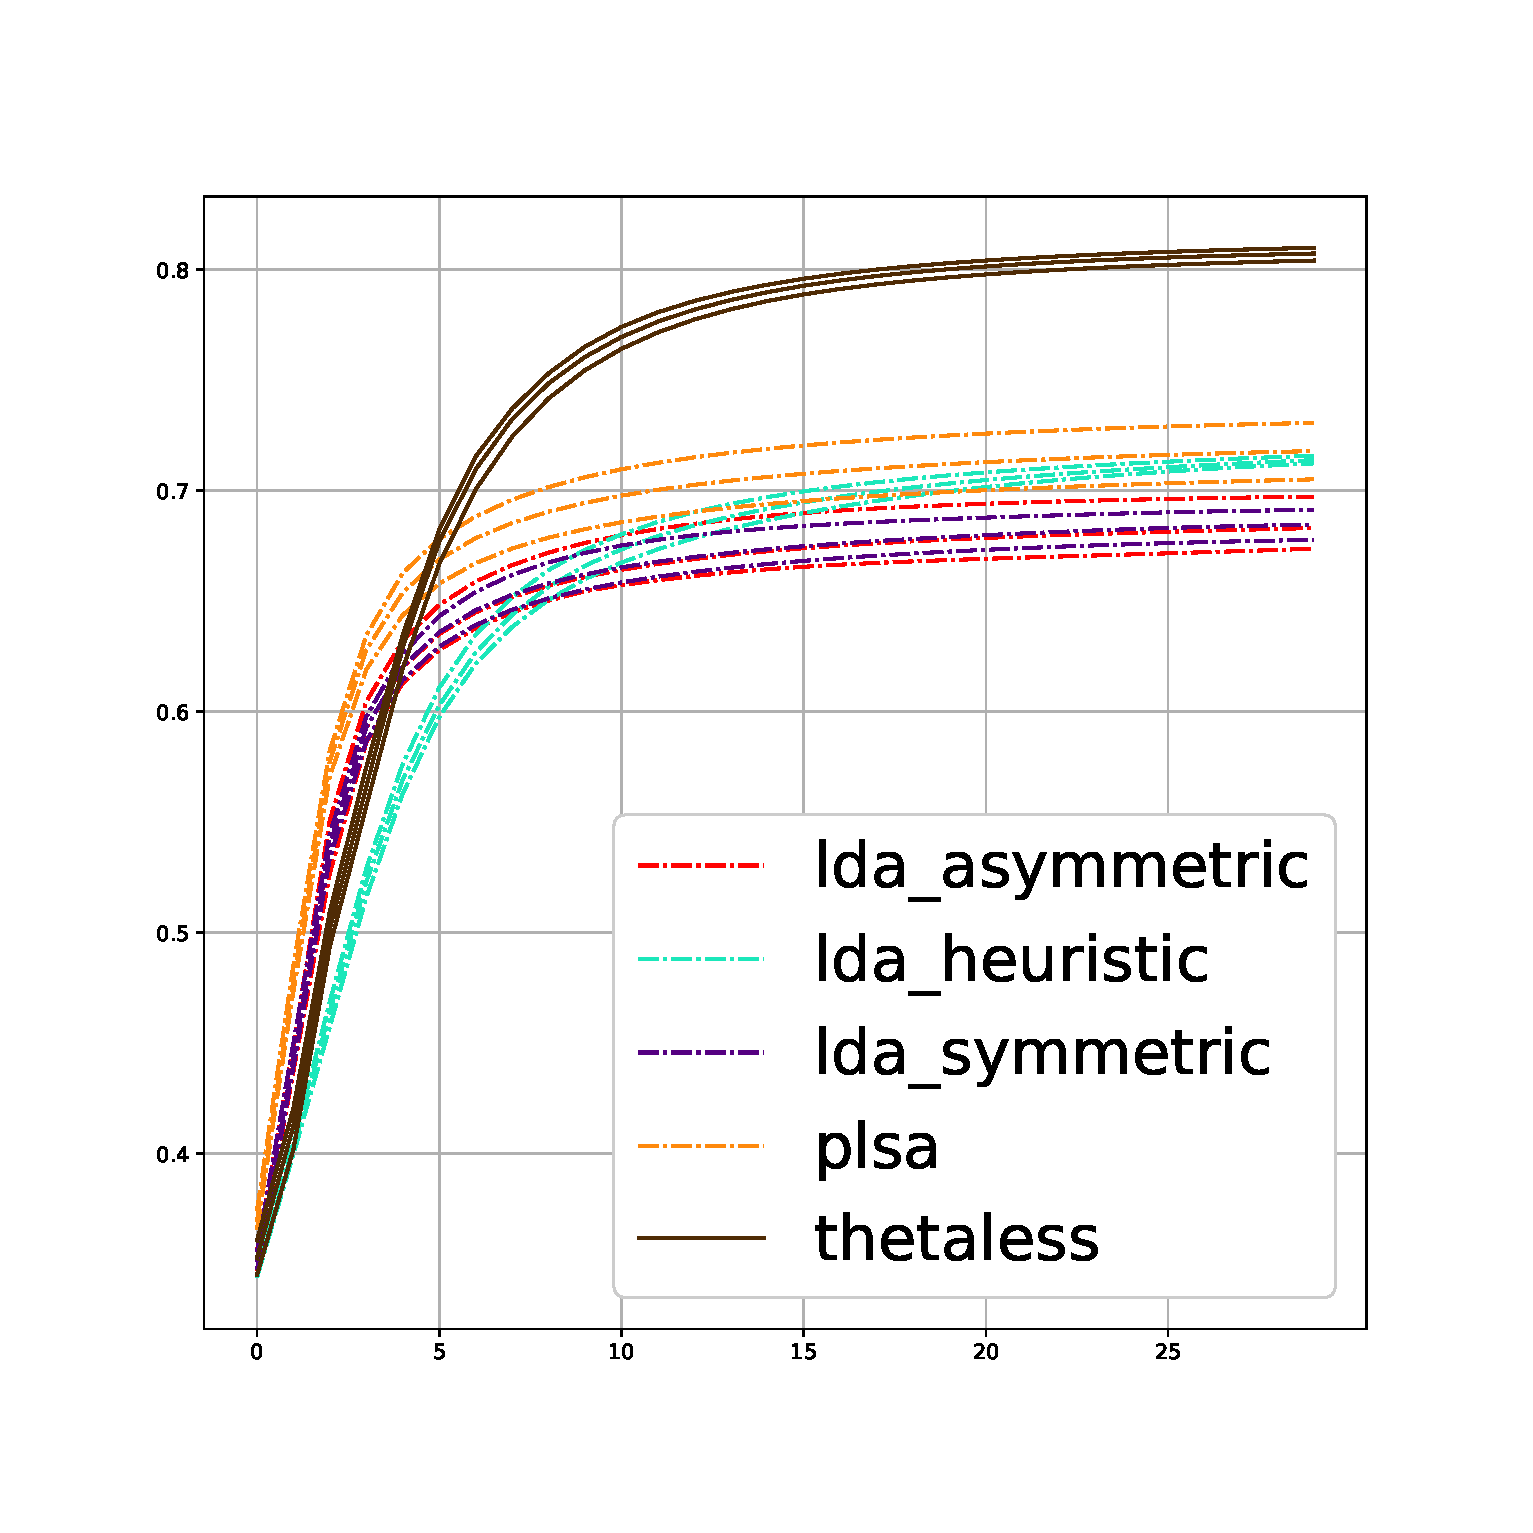
\includegraphics[width=54mm]{images/CH4_baselines_diversity_jensenshannon_False.eps}
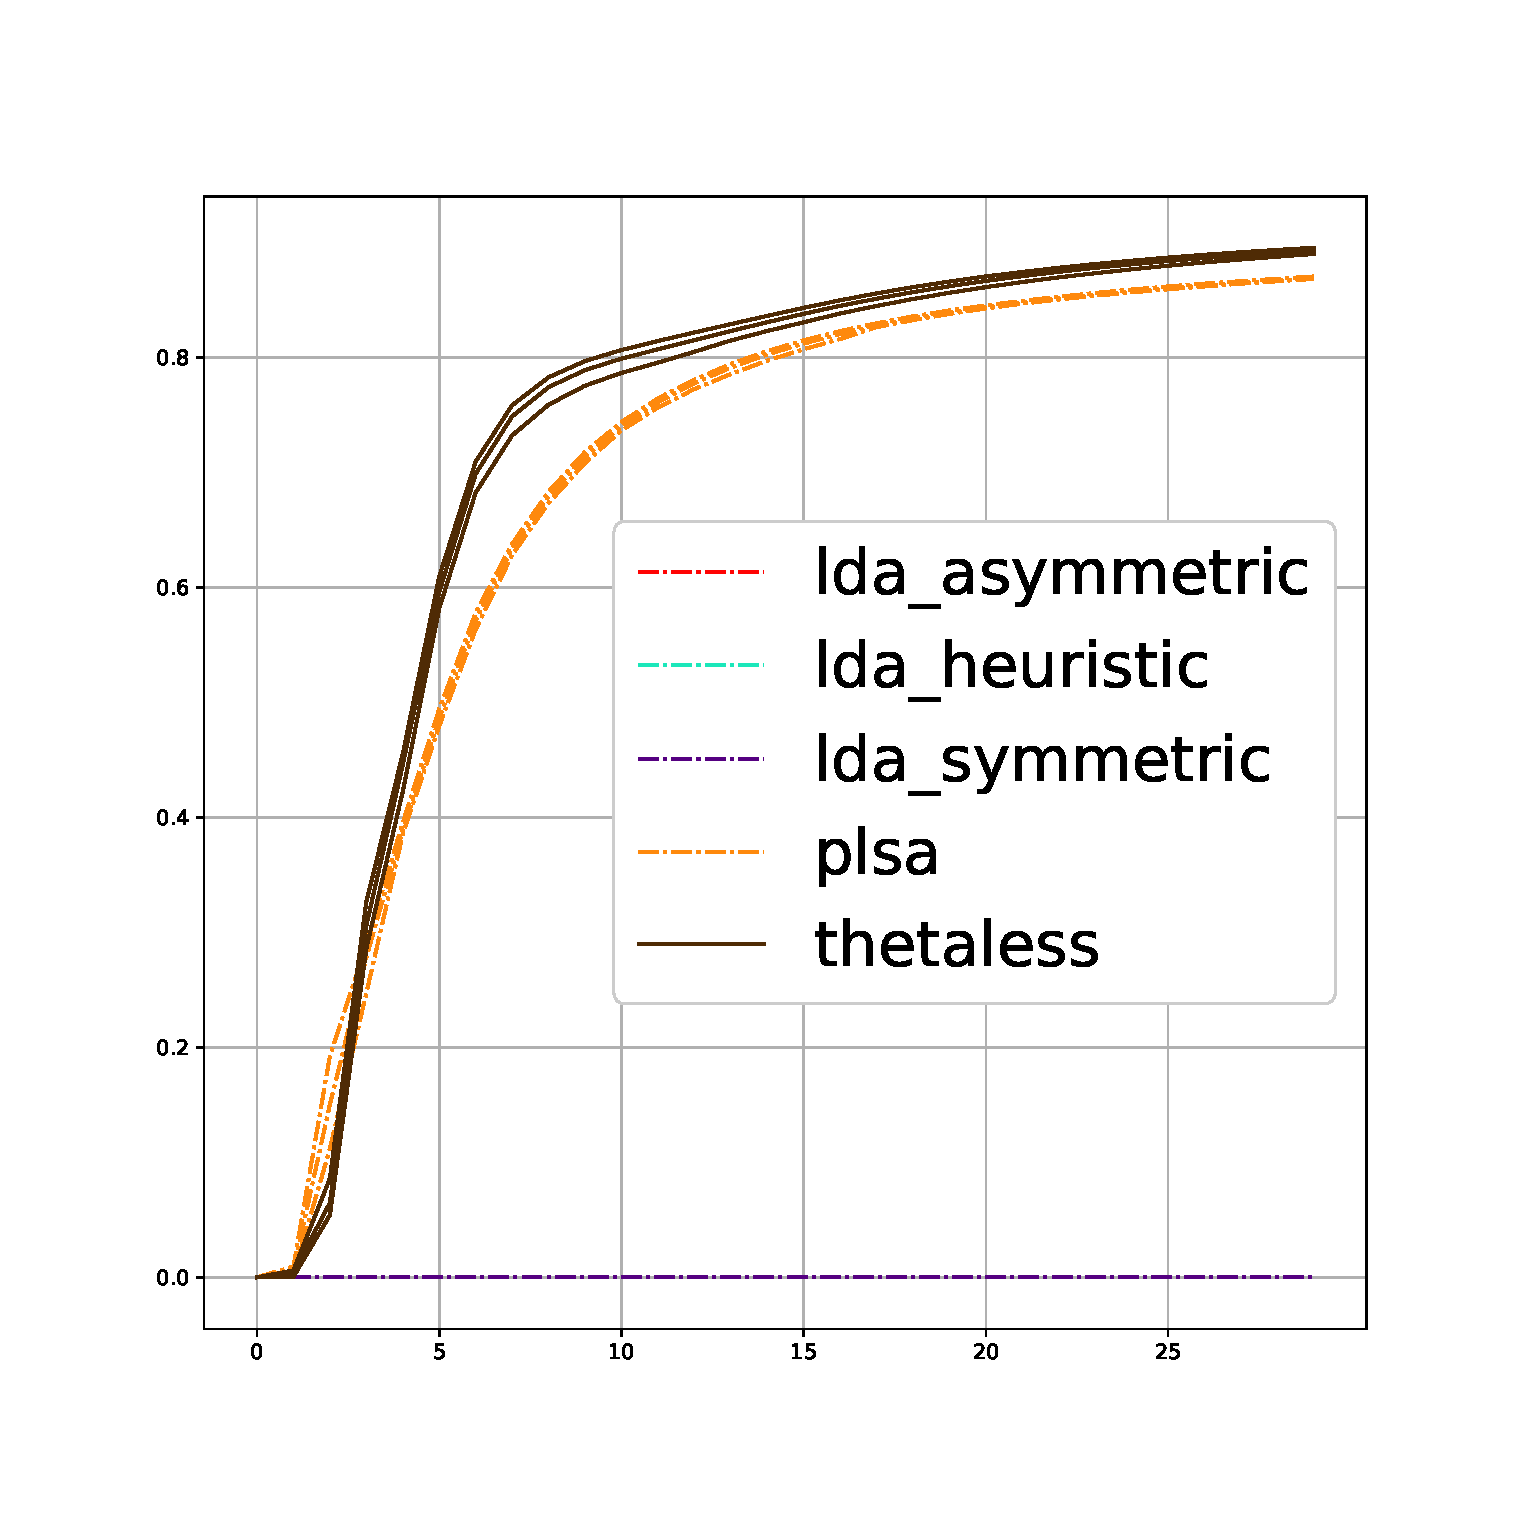
\includegraphics[width=54mm]{images/CH4_baselines_SparsityPhiScore.eps}& \end{tabular}
\end{figure}
Сравнение с базовыми моделями (PLSA и LDA с 3 видами приоров). Каждой модели соответствуют три линии: среднее значение, минимум и максимум (по пяти случайным перезапускам)
\end{frame}

\begin{frame}{Влияние на тематическую модель}

\begin{figure}
\setlength\tabcolsep{0pt} % default value: 6pt
\begin{tabular}{cc}
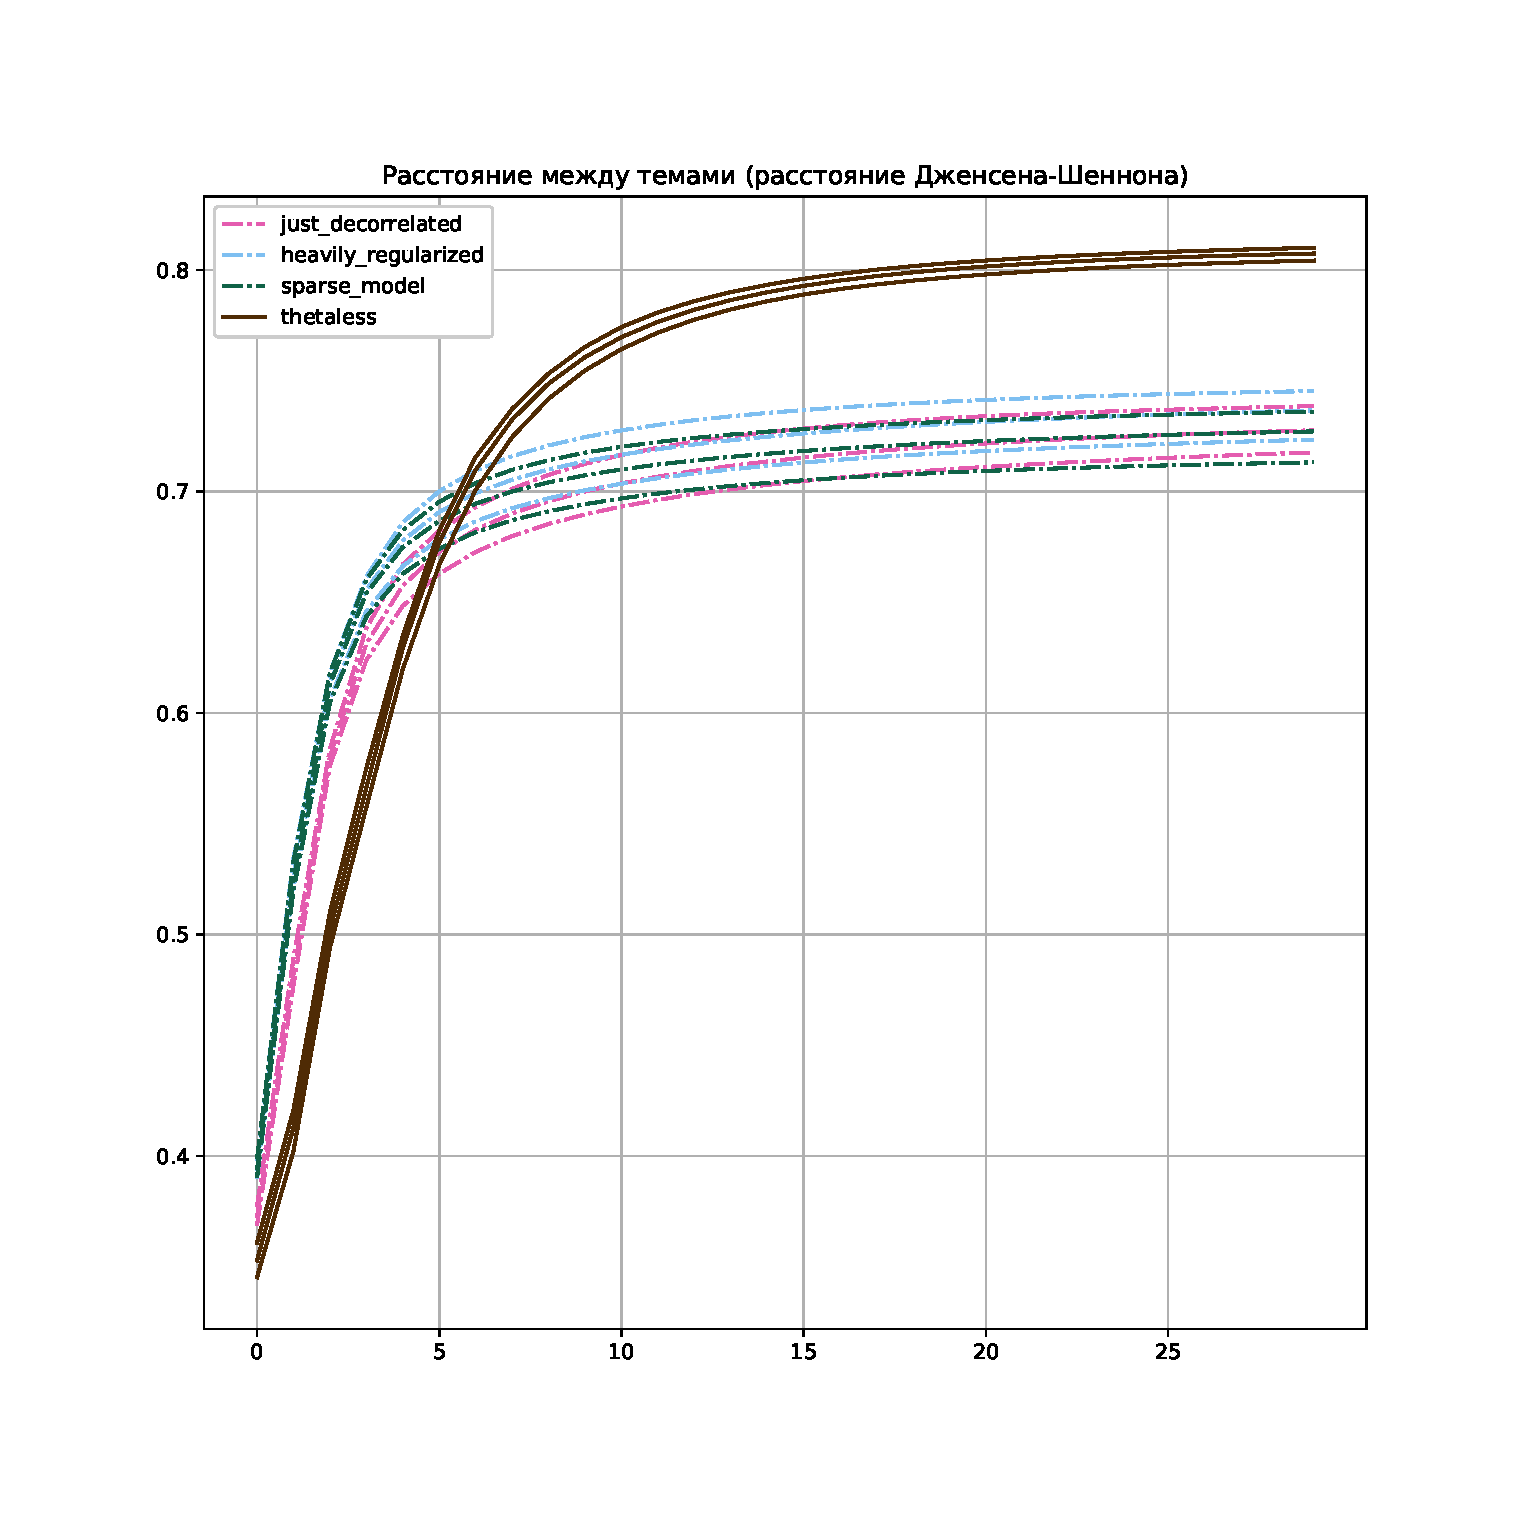
\includegraphics[width=54mm]{images/CH4_vs_regularized_diversity_jensenshannon_False.eps}
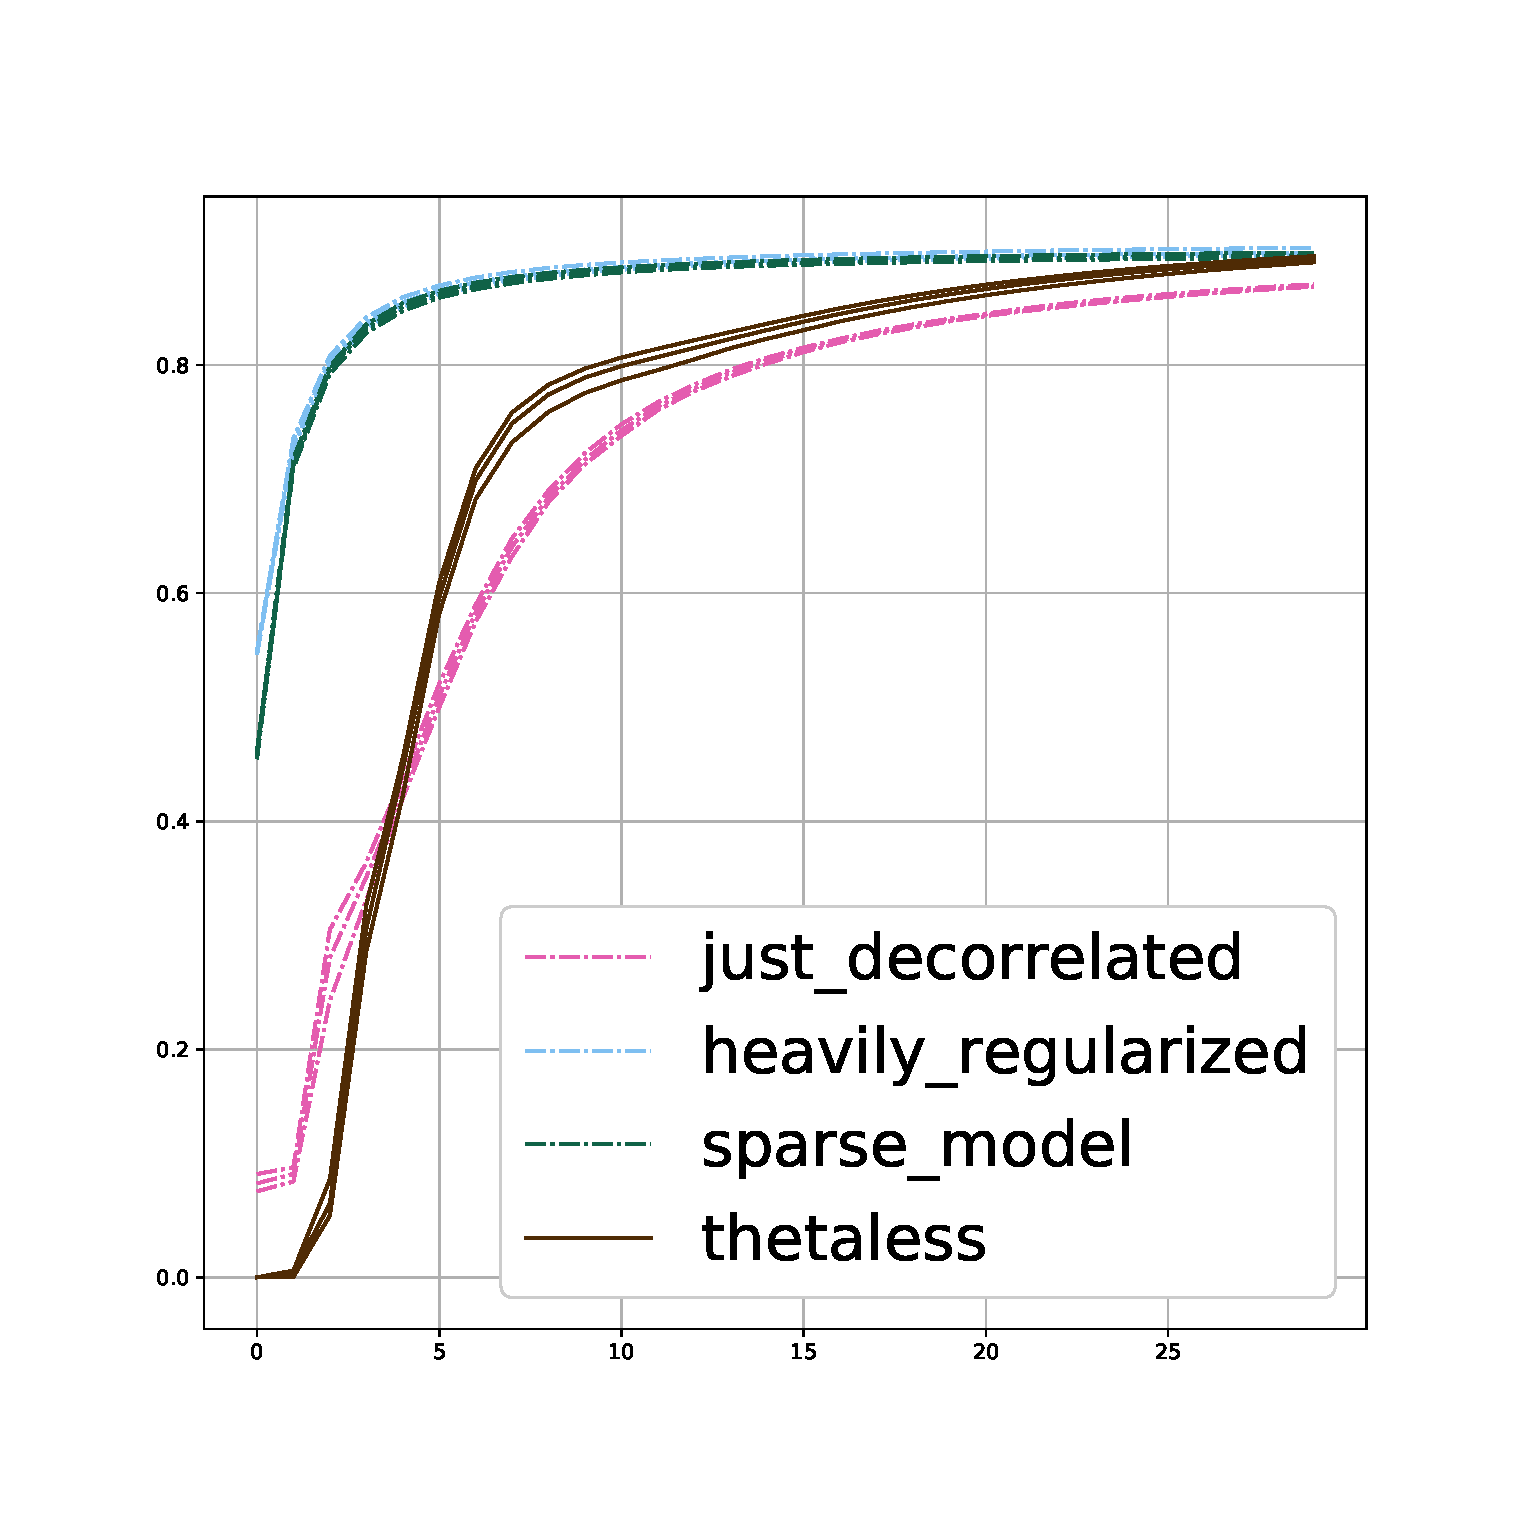
\includegraphics[width=54mm]{images/CH4_vs_regularized_SparsityPhiScore.eps}& \end{tabular}
\end{figure}
Сравнение с тремя аддитивно регуляризованными моделями
\end{frame}

\begin{frame}{Комбинирование с другими регуляризаторами}

\begin{figure}[t]
\setlength\tabcolsep{0pt} % default value: 6pt
\begin{tabular}{cc}
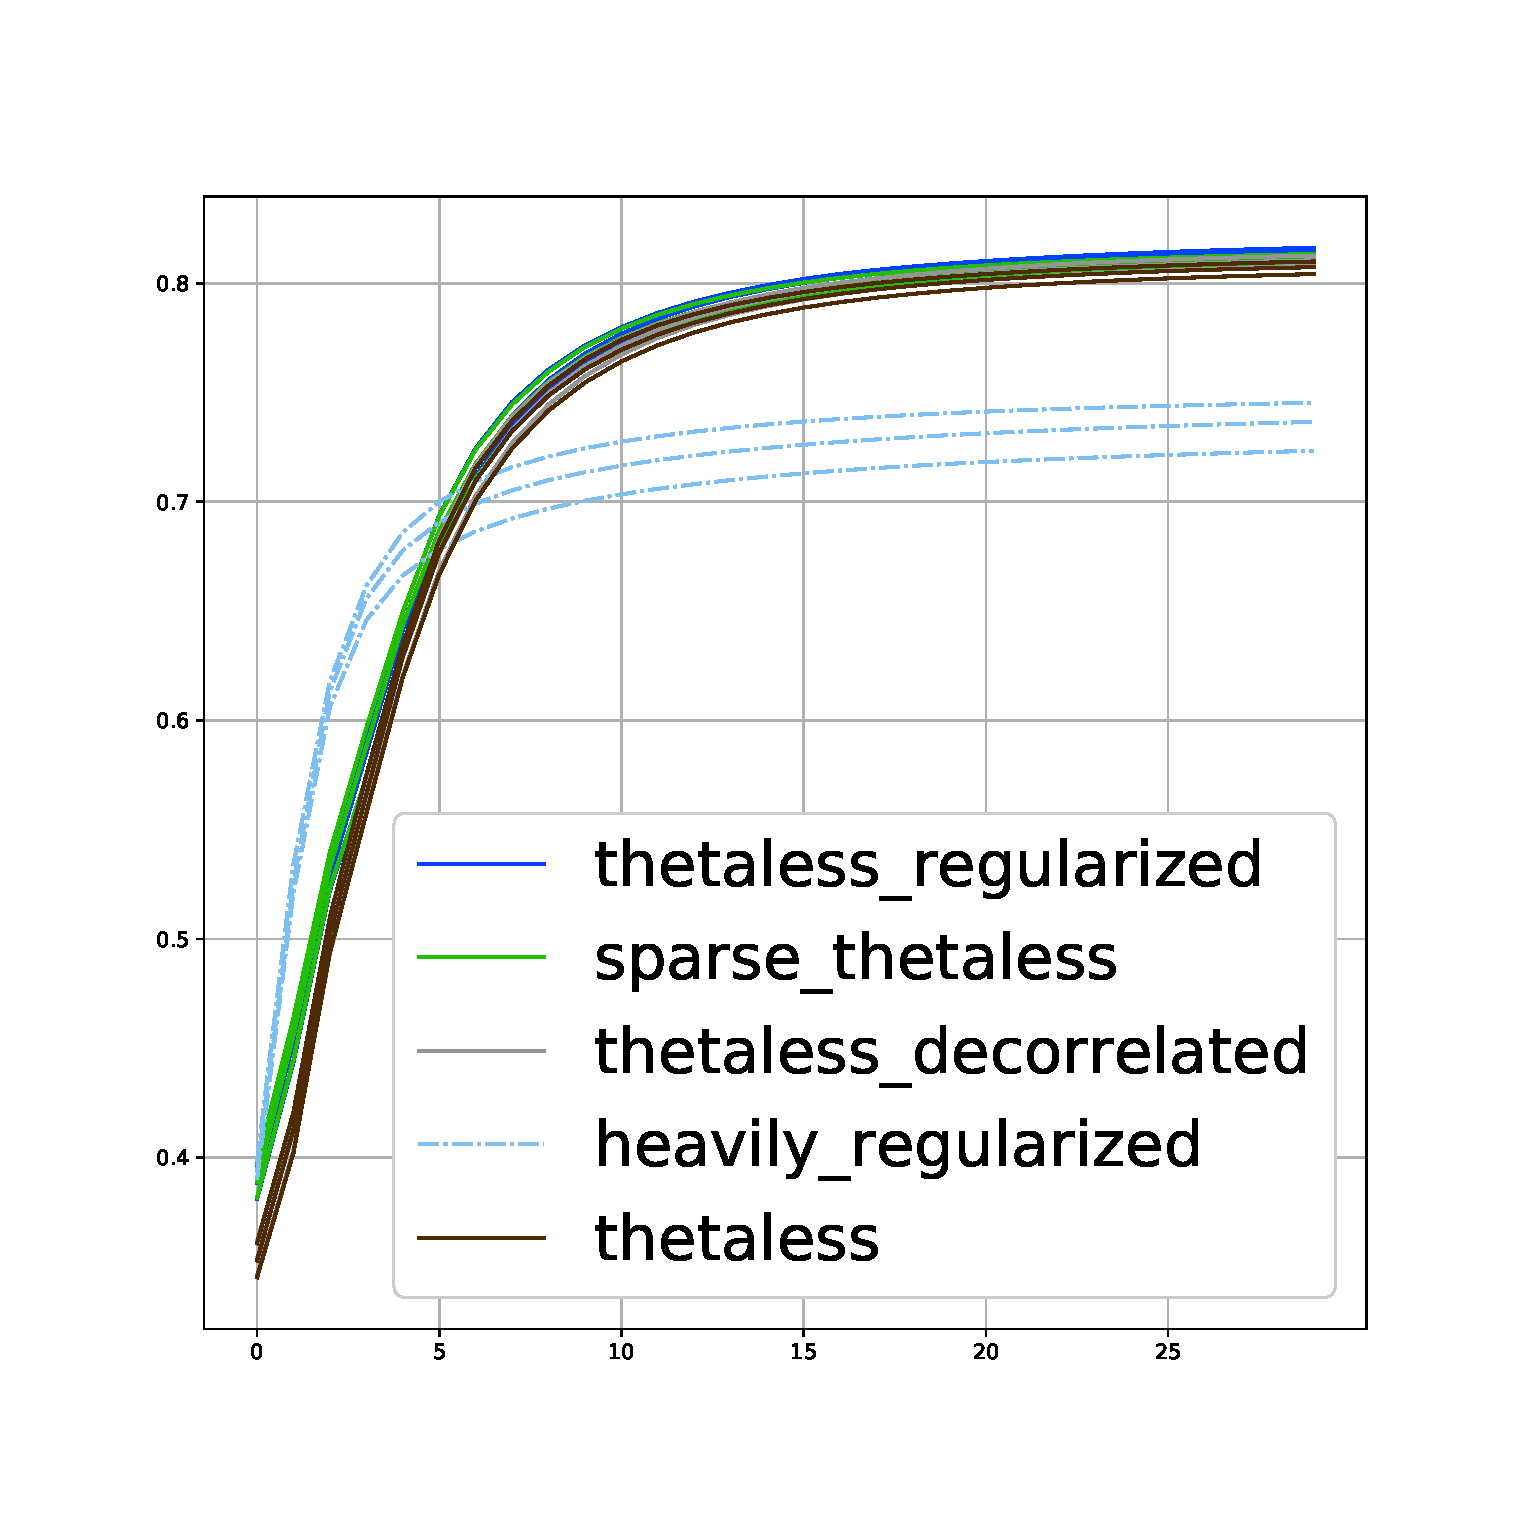
\includegraphics[width=54mm]{images/CH4_improved_diversity_jensenshannon_False.eps}
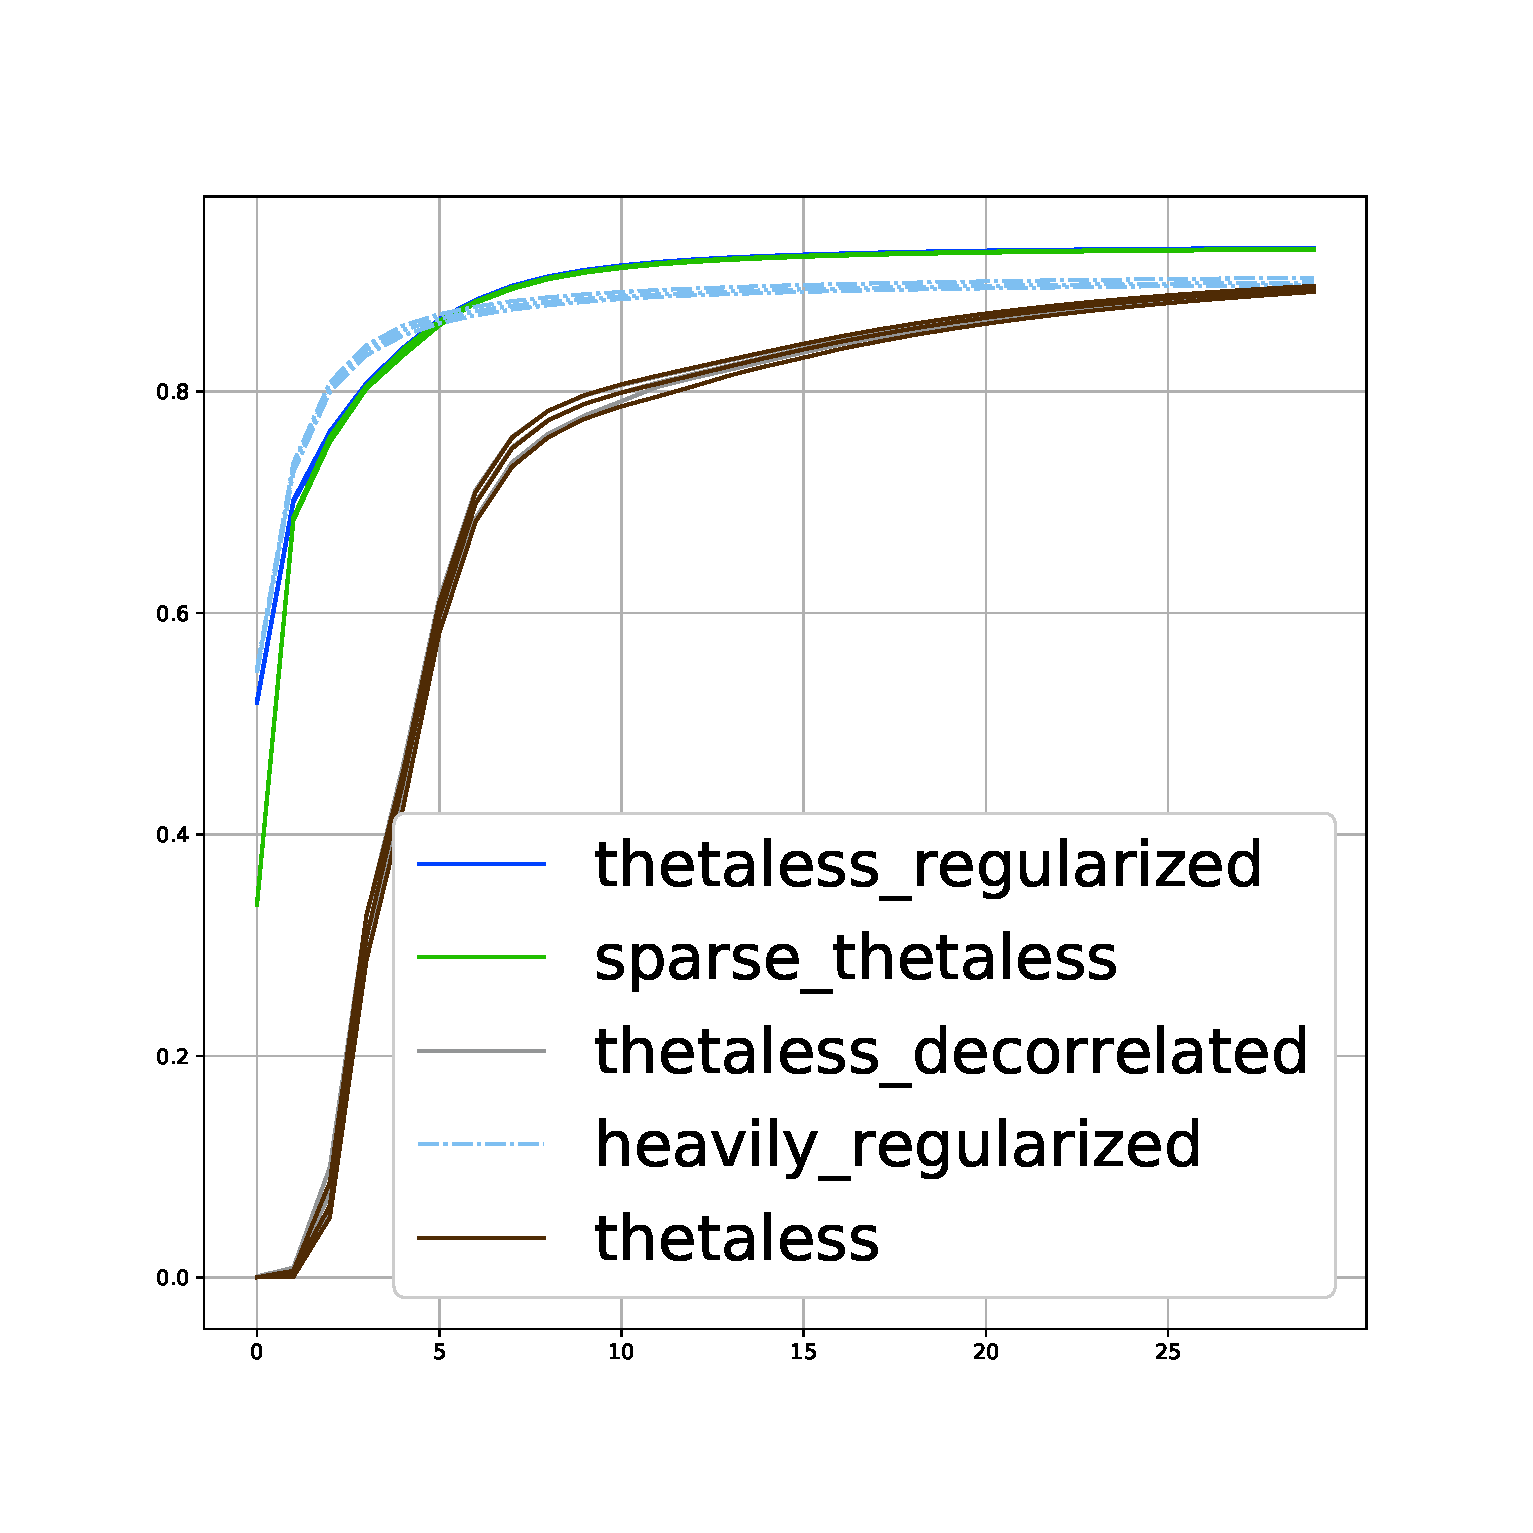
\includegraphics[width=54mm]{images/CH4_improved_SparsityPhiScore.eps}& \end{tabular}
\end{figure}
% Псевдорегуляризатор успешно комбинируется с другими регуляризаторами ARTM, за счёт чего можно улучшить критерии качества ещё больше.

Тематическая модель с псевдорегуляризатором и традиционным набором регуляризаторов (сглаживание фоновых тем, разреживание предметных тем, декорреляция) выигрывает у аналогичного ARTM по разреженности.

\end{frame}

% \BeginSection{TopicNet и <<настройки по умолчанию>>}

\begin{frame}{Базовый рецепт с быстрой векторизацией}

\begin{table}[h]
\begin{tabular}{|l|l|l|}
\hline
                         & UMass & LogLift             \\ \hline
BaselineRecipe           & -3.145         & 29.217         \\ \hline
ThetalessBleiLafferty   & -2.075         & 31.143           \\ \hline
ThetalessLift           & \textbf{-1.805}  & \textbf{33.904} \\ \hline
LDA\_asymmetric\_symmetric & -2.446          & 21.388           \\ \hline
LDA\_asymmetric\_auto      & -3.078          & 24.321          \\ \hline
LDA\_symmetric\_symmetric  & -2.884          & 23.554         \\ \hline
LDA\_symmetric\_auto       & -2.279         & 21.738          \\ \hline
LDA\_auto\_symmetric       & -2.382           & 24.154          \\ \hline
LDA\_auto\_auto            & -2.749          & 25.458 \\ \hline
\end{tabular}
\caption{Сравнение моделей по ряду критериев качества. Повышение как UMass-когерентности так и LogLift означает улучшение модели. Также модели TopicNet превосходят GenSim по разреженности и различности тем.}
\label{tbl:better_baseline}
\end{table} 

\end{frame}



\begin{frame}
    \frametitle{Положения, выносимые на защиту}
\small
    \begin{itemize}
\item
    Методология построения тематических моделей, обеспечивающая формирование <<рецептов моделирования>> с автоматизированным подбором гиперпараметров по множеству критериев и отличающаяся использованием относительных коэффициентов регуляризации и кубов гиперпараметров.
\item
    Архитектура библиотеки TopicNet, обеспечивающая программную реализацию данной методологии и отличающаяся использованием удобного языка описания кубов гиперпараметров и возможностью создания пользовательских регуляризаторов и метрик качества на языке Python.
\item
    Универсальный рецепт моделирования, обеспечивающий многокритериальный выбор тематических моделей для широкого класса задач, отличающийся предварительной настройкой куба гиперпараметров по набору разнородных задач тематического моделирования.
\item
    Программная реализация нового критерия когерентности, обеспечивающая его эффективное вычисление и отличающаяся более полным использованием данных о сочетаемости слов внутри текстовых документов.
%\item
%    Программная реализация псевдорегуляризатора в библиотеке TopicNet, обеспечивающего быстрое однопроходное вычисление тематических векторных представлений документов и улучшение качества тематической модели по множеству критериев.
    \end{itemize}

    
\end{frame}


\begin{frame}[t]{Публикации и РИДы}
\footnotesize

Публикации в изданиях, индексируемых Scopus:
\begin{itemize}
    \smallskip\item  V. Alekseev, V. Bulatov, K. Vorontsov. Intra-text coherence as a measure of topic models’ interpretability  // Dialogue 2018

    \smallskip\item A. Popov, V. Bulatov, D. Polyudova, E. Veselova. Unsupervised dialogue intent detection via hierarchical topic model // RANLP 2019

    \smallskip\item V. Bulatov, V. Alekseev, K. Vorontsov, D. Polyudova, E. Veselova, A. Goncharov, E. Egorov. TopicNet: Making Additive Regularisation for Topic Modelling Accessible // LREC 2020

    \smallskip\item\color{red} И. А. Ирхин, В. Г. Булатов, К. В. Воронцов. Аддитивная регуляризация тематических моделей с быстрой векторизацией текста // Компьютерные исследования и моделирование, 2020
\end{itemize}

Зарегистрированные программы для ЭВМ в РФ:
\begin{itemize}
    \smallskip\item  Topic Net Cooking Machine  / Гончаров А. В., Булатов В. Г., Воронцов. К. В.; МФТИ. --- опубл. 17.09.2019, 2019662102

    \smallskip\item Система создания таксономии текстовой коллекции диалогового контактного центра / Гончаров А. В., Егоров. Е. О., Веселова. Е. Р., Булатов. В. Г.; МФТИ. --- опубл. 17.03.2020, 2020613851

    \smallskip\item Topic Net Viewers  / Гончаров А. В., Булатов В. Г., Воронцов. К. В.; МФТИ. --- опубл. 10.09.2019, 2019661840

\end{itemize}

\normalsize
\end{frame}
